\documentclass[a4paper,12pt]{report}

\usepackage[utf8]{inputenc} % damit auch äöüß gehen
\usepackage[T1]{fontenc}	% so kann man bessere wörtliche rede machen
\usepackage[ngerman]{babel} % deutsche Silbentrennung
\usepackage{gensymb} % für besondere Symbole wie zB Grad -> \degree

\usepackage{csvsimple} % for tables

\usepackage{graphicx}

\usepackage{enumitem} % um aufzählungen zu machen
\usepackage[
	colorlinks,
	pdfpagelabels,
	bookmarksopen = true,
	bookmarksnumbered = true,
	linkcolor = black,
	plainpages = false,
	hypertexnames = false,
	citecolor = black
]{hyperref} % verlinkt referenzen für die digitale verwendung



%TODO: Einführung, Gruppenfoto (mit Auto), Passiver Schreibstil, Bilder, Allgemeine Beschreibungen der Kapitel, Autor der jeweiligen Funktion, Fazit, Zwischenfazit für jedes Kaptiel?, Sinnabschnitte,  Literatur/Quellverzeichnis



\begin{document}
	
%%%%%%%%%%%%%%%%%%%%% HEADER %%%%%%%%%%%%%%%%%%%%%

	\title{Robotik Praktikum -- Gruppe 2}
	\author{Frauke Jörgens (minf101207) \and Franz Wernicke (ite101729) \and Thorger Dittmann (ite101646) \and Jan Ottmüller (tinf101737) \and Felix Maaß (ite101754)}
	\date{\today}
	\maketitle
	
	\tableofcontents
	

%%%%%%%%%%%%%%%%%%%%%%%%%%%%%%%%%%%%%%%%%%%%%%%%%%	
\chapter{Allgemeine Themen}
\section{Lineare Funktion}

	Für manche Werte war es nötig eine Modulation hinzufügen zu können.
	
	Es wurde sich aus Gründen der besseren Visualisierung für einen eigenen ADTF Filter entschieden.
	Dieser nimmt ein Eingangssignal entgegen, welches daraufhin mit einem Gain und Offset versehen wird und anschließend den modulierten Wert zurückliefert.
	
	Diese Funktionalität entspricht einer "Linearen Funktion":
	
	\[y = g \cdot x + o\]
	
	wobei $x$ der Eingang, $g$ der Gain, $o$ der Offset und $y$ der Ausgang ist.
	\\
	Gain und Offset können hierbei sowohl über eigene Eingangspins als auch über variable Filterparameter gesetzt werden.

\subsection{In Entwicklung}

	Es ist geplant, dass die Geschwindigkeit des Autos mithilfe des aktuellen Lenkwinkels in Kurven angepasst werden kann.

%%%%%%%%%%%%%%%%%%%%%%%%%%%%%%%%%%%%%%%%%%%%%%%%%%
\chapter{Lenkung}

%TODO: Hier ein bisschen was über die beiden Filter schreiben + Ackermann Steering Approximation + Theoretische Überlegungen auf zettel und papier
%https://en.wikipedia.org/wiki/Steering

%%%%%%%%%%%%%%%%%%%%%%%%%%%%%%%%%%%%%%%%%%%%%%%%%%
\chapter{Motorregelung}	

%%%%%%%%%%%%%%%%%%%%%%%%%%%%%%%%%%%%%%%%%%%%%%%%%%
\chapter{Kollisionsvermeidung}

	Mithilfe der Ultraschallsensoren sind vorn und hinten Hindernisse zu erkennen.
	Dadurch soll es möglich sein, zu reagieren bevor eine Kollision stattfindet.

\section{Genauigkeit der Ultraschallsensoren}

	\paragraph{Situation.}
	Die Ultraschallsensoren liefern einzeln betrachtet recht akkurate Werte.
	Die Genauigkeit wurde zu $\pm1cm$ bestimmt.
	
	\paragraph{Problem.}
	Leider ist es jedoch der Fall, dass die Messungen Ausreißer aufweisen.
	Teils wurden leicht erkennbare Fehler zurückgegeben ($-1$). Teils wichen die Werte aber auch um erhebliche Beträge ab.
	
	Den Grund für Letzteres diagnostizierten wir in der gleichzeitigen Ansteuerung der Sensoren.
	Da jedoch der Code der Arduinos (welche sich um die Erfassung der Werte kümmern) nicht offen liegt und für uns somit anpassbar wäre, können wir vorerst keine Änderungen daran vornehmen.
	
	Damit diese falschen Werte dennoch nicht mit in kommende Berechnungen einbezogen werden, musste eine entsprechende Lösung gefunden werden.

	\paragraph{Resultat.}
	Zur Stabilisierung der Messwerte entschieden wir uns für eine Filterung.
	Es wurde nach einem Filter gesucht, der robust gegenüber Ausreißern ist.
	Hier kam uns als Erstes der Median in den Sinn.
	
	Ein entsprechender Filter wurde nun sowohl als C++ Klasse als auch als ADTF Filter erstellt.

	Der ADTF Filter besitzt einen Parameter, der die Fenstergröße einstellt (i.e. die Anzahl an Werten über die der Median gebildet werden soll) und ermöglicht damit eine flexible Filterung der Messwerte.

\section{Hinderniserkennung}
	
	Mithilfe der aufbereiteten Ultraschallsensordaten wird es möglich sein, das Auto sicher durch die Umgebung zu navigieren.
	\footnote{Dieses Feature befindet sich noch in Entwicklung.}
	
\subsection{Theoretische Überlegungen}
	
	Um sich ein geeignetes Bild der Umgebung zu machen, ist es sinnvoll, jeden  Messwert der fünf Frontsensoren einzeln zu bewerten, da sonst unnötige Manöver eingeführt werden, um Objekten auszuweichen, die nicht auf unserer Trajektorie liegen.
	Uns erschien es sinnig, dies anhand des aktuellen Lenkwinkels zu tun.
	
	Es wurde eine Funktion synthetisiert, die die Relevanz der einzelnen Messwerte zu dem Lenkwinkel in Relation setzt:
	
		\[y=2-e^{-3 \cdot \left( x-a \right)^2}\]
	
	Sie bietet eine Gewichtung für Messwerte der jeweiligen Sensoren.
	Hierbei steht $x$ für den Montagewinkel des zu gewichtenden Sensors, $a$ für den aktuellen Lenkwinkel und $y$ für die Gewichtung (den Skalierungsfaktor).
	
	Dies bewirkt, dass Messwerte von Sensoren, die nicht in Fahrtrichtung zeigen, weniger stark in die Hinderniserkennung mit eingehen, ohne diese gänzlich ausschließen zu müssen.
	
	\paragraph{Veranschaulichung.} \autoref{img_uss_function} zeigt die Funktion bei $a = 0\degree$ Auslenkung.
	Das Minimum der Kurve befindet sich stets bei dem aktuellen Lenkwinkel, da hier gilt: $x = a$.
	
	Die blauen Vertikalen zeigen Hilfslinien bei $45\degree$ Montagewinkel.
	
	
	\begin{figure}
		\centering
		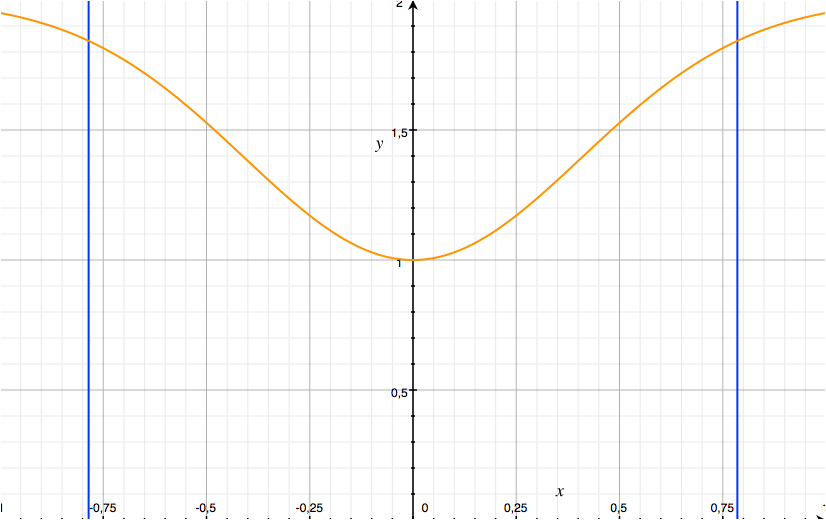
\includegraphics[width=\textwidth,height=\textheight,keepaspectratio]{assets/uss-function}
		\caption{Gewichtungsfunktion für einen Lenkwinkel von $a = 0\degree$}
		\label{img_uss_function}
	\end{figure}
	

%%%%%%%%%%%%%%%%%%%%%%%%%%%%%%%%%%%%%%%%%%%%%%%%%%
\chapter{Kollisionserkennung}

	Mithilfe der Daten des Accelerometers werden Kollisionen erkannt und ein sofortiger Nothalt ausgelöst.
	\footnote{Dieses Feature befindet sich noch in Entwicklung.}
	
	Dabei wird darauf geachtet, dass die Ausschläge der Werte entsprechend hoch und kurzweilig sind, da auch bei starkem Abbremsen bereits starke aber anhaltende Beschleunigungen entstehen.
	

%%%%%%%%%%%%%%%%%%%%%%%%%%%%%%%%%%%%%%%%%%%%%%%%%%	
\chapter{Fahrbahnerkennung}

\section{Linienerkennung (Binarisierung)}
	Threshold, HSV-Modell, Closing, ...

\section{Canny Edge Detection} %TODO vorher/nachher Bilder

\section{Hough Line Transformation}

\section{Line-Clustering}

\section{Klassifizierung}

\subsection{Haltelinien}

\section{Zentrierung in der Fahrspur}
	
	Bisher ist das Auto in der Lage der Fahrspur zu folgen.
	Allerdings besteht das Problem, dass es sich nicht in der Mitte der Spur zentriert.
	Dies führt dazu, dass es oft bereits auf den Linien fährt und teilweise sogar die andere Fahrspur mitbenutzt.
	Da dies sicher kein erwünschtes Verhalten ist behandelt dieser Abschnitt unsere Herangehensweise.

\subsection{Theoretische Überlegungen}

	Angenommen es werden zwei Linien (linke und rechte Leitlinie) erkannt.
	Es wird nun jeweils der Abstand zur Seite ermittelt und dann gemittelt (Arithmetisches Mittel).
	Das Ergebnis ist ein Wert, der entweder links, rechts oder genau auf der Ideallinie des Fahrspur liegt.
	
	Es wird nun eine Funktion gesucht, die die Abweichung in eine Lenkanweisung umsetzt.
	Da dies schnell zu instabilen Verhalten führen kann, fällt eine lineare Funktion raus.
	Hier würde zu oft nachkorrigiert werden müssen.
	
	Unsere Wahl fiel dabei auf eine modifizierte Sigmoid-Funktion:
	\footnote{Die Funktion wird symmetrisch auch für Abweichungen nach links eingesetzt. Hierbei muss lediglich das Vorzeichen beachtet werden.}
	
		\[y=\frac{a_{max}}{1 + e^{-14\left( \frac{x}{x_{max}}-\frac{1}{2} \right)}}\]
	
	Hierbei steht $x$ für die aktuelle und $x_{max}$ für die maximale Abweichung von der Ideallinie.
	Der maximal anzusteuernde Lenkwinkel wird durch den Parameter $a_{max}$ angegeben.
	
	\paragraph{Veranschaulichung.} \autoref{img_spurzentrierung_function} zeigt die Funktion beispielhaft für $a_{max} = x_{max} = 1$, also in ihrer normierten Darstellung.
	
	Je weiter das Auto sich also von der Ideallinie entfernt, desto stärker wird der Lenkeinschlag und somit der Drang sich wieder zu zentrieren.
	
	Durch das exponentielle Verhalten ist sichergestellt, dass ein Aufschwingen nicht möglich ist. Es existiert eine Art Totzone.
	
	\begin{figure}[ht]
		\centering
		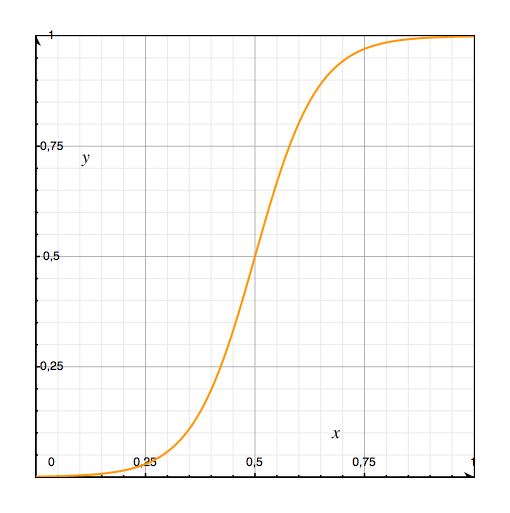
\includegraphics[width=200pt,keepaspectratio]{assets/spurzentrierung}
		\caption{Normierte Spurzentrierung}
		\label{img_spurzentrierung_function}
	\end{figure}
	
	
\end{document}


